% https://tex.stackexchange.com/questions/129629/how-can-i-get-a-stacked-bar-with-single-values-and-sum-on-top
\documentclass[border=5mm] {standalone}
\usepackage{pgfplots, pgfplotstable}

\begin{document}
  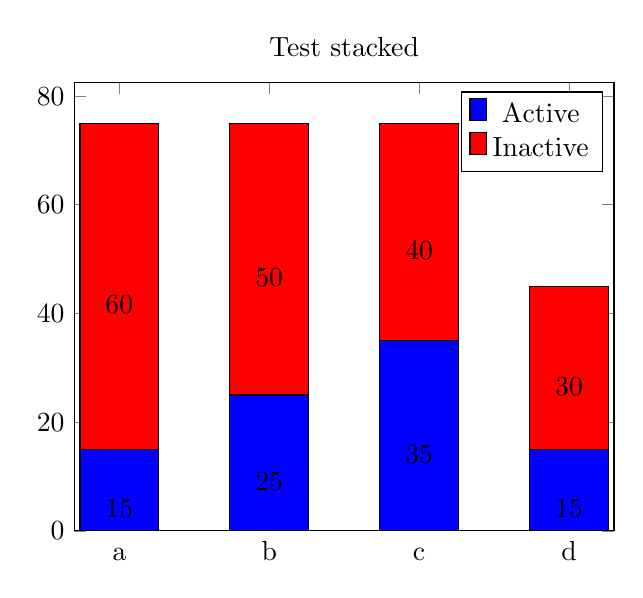
\begin{tikzpicture}
  \begin{axis}[
    title={Test stacked},
    ybar stacked, ymin=0,  
    bar width=10mm,
    symbolic x coords={a,b,c,d},
    xtick=data,
    nodes near coords, 
    nodes near coords align={anchor=north},%Move values in bar
    totals/.style={nodes near coords align={anchor=south}},
    x tick label style={anchor=south,yshift=-0.5cm},
  ]
  %Active
  \addplot [fill=blue] coordinates {
({a},15)
({b},25)
({c},35)
({d},15)};
  %Inactive
  \addplot [fill=red,point meta=explicit] coordinates {
({a},60) [60]
({b},50) [50]
({c},40) [40]
({d},30) [30]};
  \legend{Active,Inactive}
  %Dummy stacked plot to produce totals
  \addplot[totals] coordinates {
({a},0)
({b},0)
({c},0)
({d},0)};
  \end{axis}
  \end{tikzpicture}
\end{document}